\chapter{Achieving the Highest Processing Power} \label{chap:sota1}
%Estado da arte (escolher um nome que capte o domínio do trabalho)
%Trabalhos relacionados, tecnologias existentes, abordagens ao problema ou a problemas %semelhantes
\section*{}

The introduction describes a brief overview about each content of each chapter that this report is made up with. This chapter will focus on the state of the art in how to achieve the highest processing power. Related work and already known technologies are the main point in this chapter.  


\section{Introduction}

Following the context introduced in the previous chapter, the idea of having different processing components in a computer system doesn't improve the applications performance on its own. This is where the developers' work is crucial to take advantages of such different systems. The developers' work is to schedule the application's tasks to the different components so that these components can work simultaneously, avoiding overheads caused by their parallel activity, accessing memory at the wrong moment, memory conflicts, task dependency, wrong application's results compared with the sequential application.~\cite{Lee}

As mentioned previously, trying to create parallelized code can arise many problems and must be handled so the applications don't lose their functionalities. In order to do so, it requires a lot of time and effort to make it correctly parallelized. So trying to make code parallelization automatic is the next step in the direction of taking the most advantage of heterogeneous systems which, consequently, improves applications performance. 

This chapter is divided in two parts: one part will focus in the system's heterogeneity, how they can be used in favor of enhancing performance; and the main point of the other part is taking advantage of parallel activity by transforming sequential code into parallelized code.


\section{Using Computers' Heterogeneous Components}\label{sec:dialecto}

Technologies and frameworks in this field have been developed in order to manipulate and control efficiently the different processing components. The main goal of this technologies is to optimize application parallelization; application memory management; application workload; application scheduling queue and application kernel dimension.

An interesting fact is that the following software/frameworks that will be present are built, as its bases, under OpenCL programing language due to the fact that this language's use is targeted to heterogeneous parallel programing with CPUs and GPUs.

\subsection{OpenCL}
OpenCL is a programming language for heterogeneous parallel programing targeted to CPUs, GPUs and other processors~\cite{Shen}. In a small brief,  this language is designed to take advantage of different types of processors and facilitates heterogeneous computing integration in applications' code. The user programs in a virtual platform and the source code that has been developed there is compatible for any system that supports OpenCl. Additionally, OpenCL allows users to control the applications' tunning parallelism through its hardware abstraction. In figure~\ref{fig:opcl} there is an idea of the OpenCL plataform model and memory model for a better understanding of this hardware abstractions that was previously mentioned.

The OpenCL's programs has two parts: the compute kernels that are executed depending the number of processing  devices; and the program that will be run. The program creates a set of commands and puts them in a queue for each device, additionally, to manage the execution of each kernels, additional commands are queued in the different kernels. When the computation is finished, the result data, from the previous kernels activity, return back to the original program. 

\begin{figure}[t]
  \begin{center}
    \leavevmode
    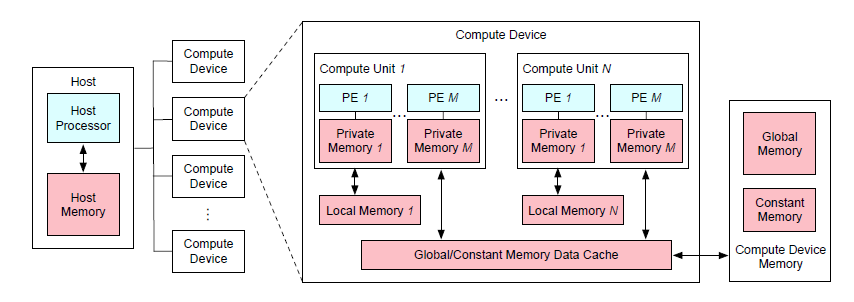
\includegraphics[width=1\textwidth]{OpenCL}
    \caption{The OpenCL platform model and the OpenCL memory model}
    \label{fig:opcl}
  \end{center}
\end{figure}

%\subsection{Cooperative Heterogeneous Computing (CHC) framework}
%~\cite{Lee}
\subsection{StarPU}
StartPU is a software tool with the purpose for programmers to use the computing power available in CPUs and GPUs, wihtout needing to care about if their programs are adapted to a specific machine and its processing components.~\cite{StartPU}
In fact, StartPU is a run-timpe support library that provides scheduling applications-provided tasks on heterogeneous environments, such as CPUs and GPUs. Additionally, it comes with programming language support, for the programming C language extensions and for OpenCL.

Programs submit computational tasks, with CPU and/or GPU implementations, and StarPU schedules these tasks and associated data transfers on available CPUs and GPUs. The data that a task manipulates are automatically transferred among accelerators and the main memory, so that programmers are freed from the scheduling issues and technical details associated with these transfers.

StarPU takes particular care of scheduling tasks efficiently, using well-known algorithms from the literature (Task Scheduling Policy). In addition, it allows scheduling experts, such as compiler or computational library developers, to implement custom scheduling policies in a portable fashion (Defining A New Scheduling Policy).
\subsection{Twin Peaks}
"Software platform that enables applications originally targeted for GPUs to be executed efficiently on multicore CPUs", mentioned by Jayanth Gummaraju, Laurent Morichetti, Michael Houston, Ben Sander, Benedict R. Gaster, Bixia Zheng, in the paper \textit{Twin peaks: a software platform for heterogeneous computing on general-purpose and graphics processors} ~\cite{Gummaraju2010}. This is a small definition of the Twin Peaks' job. The aim of this software is, firstly, to program applications using an API written in OpenCL; secondly, to compile the applications code to, for instance, add syntactic and semantic checks to make sure that the kernels meet the OpenCL requirements; and execute applications in the heterogeneous environment using CPUs and GPUs.

\section{Using Code Parallelization}
Great advances have been made in the code parallelization. However, currently this kind of practice (the code parallelization) mostly is done by programmers and it requires a lot of effort, time and knowledge. It requires knowledge in the best practices related to what should and can't be parallelized, good knowledge on the code: its functionalities and its correct outputs because without these knowledges the chances to parallelize code correctly would be low since it is important to know if, firstly, is possible to parallelize and if, secondly, the parallelization doesn't jeopardize the programs results, outcomes and performance; to sum up, it requires time and effort to get a deep understanding of the code and to try if the code is correctly parallelized.~\cite{Jeon}

Since this practice is very costly, although grants great results at performance levels, this field has been developing ways to have results less costly, mostly in effort and time-consuming. These developments created tools to help programmers develop parallelized code, using OpenMP directives, or software tools which recommend possible parallelized regions and its theoretical speed up gain, with Kremlin, or even a way to estimate how much can a program be parallelized, with Kismet software.~\cite{Saturnino}

The following software tools that will be presented have, as its base support, OpenMP directives to help in parallelizing code, or at least, to measure performance.

\subsection{OpenMP}
OpenMP was designed to be a flexible standard, easily implemented across different platforms. the main objectives are: control structure, the data environment, synchronization, and the runtime library. 

In terms of how it really does its job, OpenMP was designed to exploit certain characteristics of shared-memory architectures. The ability to directly access memory throughout the system , combined with fast shared memory locks, makes shared-memory architectures best suited for supporting OpenMP. in practice, OpenMP is a set of compiler directives and callable runtime library routines that extend Fortran (and separately, C and C++) to express shared-memory parallelism.~\cite{Nc1998}. To be more precise, OpenMP provides standard environment variables to accompany the runtime library functions where it makes sense and to simplify  the start-up scripts for portable applications. This helps application developers who, in addition to creating portable applications, need a portable runtime environment. OpenMP has been designed to be extensible and evolve with user requirements. The OpenMP Architecture Review Board was created to provide long-term support and enhancements of the OpenMP specifications. 

\subsection{Kremlin}
The true purpose of Kremlin lies in asking the following question: "What parts of this program should I spent time parallelizing?"~\cite{ParalledSoftware}. So, in overall, Kremlin profiles a serial program and tells the programmer not only what regions should be parallelized, but also the order in which they should be parallelized to maximize the return on their effort.
Giving a non parallelized code, Kremlin guides the programmer how to achieve better performance in its program though parallelization by presenting a list of code regions that could be parallelized. this list contains a plan that will minimize the number of regions that must be parallelized to maximize the programs performance, though parallelization.

At the core of the Kremlin system is a heavyweight analysis of a sequential program’s execution that is used to create predictions
about the structure of a hypothetical, optimized parallel implementation of the program. These predictions incorporate both optimism and pessimism to create results that are surprisingly
accurate.~\cite{Garcia2011}

Overall, Kremlin is an automatic tool that, given a serial version of a program, will make recommendations to the user as to what regions (e.g. loops or functions) of the program to attack first.~\cite{Garcia2012}  

\subsection{Kismet}
Opposed to Kremlin, Kismet helps mitigate the risk of parallel software engineering by answering the question, "What is the best performance I can expect if I parallelize this program?"~\cite{ParalledSoftware}. Kismet profiles serial programs and reports the upper bound on parallel speedup based on the program's inherent parallelism and the system it will be running on.

Kismet performs dynamic program analysis on an unmodified serial version of a program to determine the amount of parallelism available in each region(e.g. loop and function) of the program. Kismet then incorporates system constrains to calculate an approximate upper bound on the program's attainable parallel speedup. ~\cite{Taylor}

In order to estimate the parallel performance of a serial program, Kismet uses a parallel execution time model. Kismet's parallel execution time model is based on the major components that affect parallel performance, including the amount of parallelism available, the serial execution time of the program, parallelization platform overheads, synchronization and memory system effects which contribute in some cases to super-linear speedups.

\section{Overview}

As mentioned before, the previously presented software tools, for both cases (using computers' heterogeneous components and using code parallelization) have their base support even being a programming language, for OpenCL, or a set of compile directives, for OpenMP. Those software tools have improved applications performance somehow, which is already good. However, looking as a software that can do everything on its own, with the minimum programmer's input, in other words, that can do things almost automatically, none of them can make it. The only software tool that is close to that automation is Kremlin because it gives what a developer should do in their code in order to increase its efficiency and performance.

Both approaches, using computers' heterogeneous components and using code parallelization, have the role to answer the state of the art premise: "achieving the highest processing power".  
